%\documentclass[twocolumn,journal]{IEEEtran}
\documentclass[onecolumn,journal]{IEEEtran}
\usepackage{amsfonts}
\usepackage{amsmath}
\usepackage{amsthm}
\usepackage{amssymb}
\usepackage{graphicx}
\usepackage[T1]{fontenc}
%\usepackage[english]{babel}
\usepackage{supertabular}
\usepackage{longtable}
\usepackage[usenames,dvipsnames]{color}
\usepackage{bbm}
\usepackage{caption}
\usepackage{fancyhdr}
\usepackage{breqn}
\usepackage{fixltx2e}
\usepackage{capt-of}
%\usepackage{mdframed}
\setcounter{MaxMatrixCols}{10}
\usepackage{tikz}
\usetikzlibrary{matrix}
\usepackage{endnotes}
\usepackage{soul}
\usepackage{marginnote}
%\newtheorem{theorem}{Theorem}
\newtheorem{lemma}{Lemma}
%\newtheorem{remark}{Remark}
%\newtheorem{error}{\color{Red} Error}
\newtheorem{corollary}{Corollary}
\newtheorem{proposition}{Proposition}
\newtheorem{definition}{Definition}
\newcommand{\mathsym}[1]{}
\newcommand{\unicode}[1]{}
\newcommand{\dsum} {\displaystyle\sum}
\hyphenation{op-tical net-works semi-conduc-tor}
\usepackage{pdfpages}
\usepackage{enumitem}
\usepackage{multicol}
\usepackage[utf8]{inputenc}


\headsep = 5pt
\textheight = 730pt
%\headsep = 8pt %25pt
%\textheight = 720pt %674pt
%\usepackage{geometry}

\bibliographystyle{unsrt}

\usepackage{float}

 \usepackage{xcolor}

\usepackage[framemethod=TikZ]{mdframed}
%%%%%%%FRAME%%%%%%%%%%%
\usepackage[framemethod=TikZ]{mdframed}
\usepackage{framed}
    % \BeforeBeginEnvironment{mdframed}{\begin{minipage}{\linewidth}}
     %\AfterEndEnvironment{mdframed}{\end{minipage}\par}


%	%\mdfsetup{%
%	%skipabove=20pt,
%	nobreak=true,
%	   middlelinecolor=black,
%	   middlelinewidth=1pt,
%	   backgroundcolor=purple!10,
%	   roundcorner=1pt}

\mdfsetup{%
	outerlinewidth=1,skipabove=20pt,backgroundcolor=yellow!50, outerlinecolor=black,innertopmargin=0pt,splittopskip=\topskip,skipbelow=\baselineskip, skipabove=\baselineskip,ntheorem,roundcorner=5pt}

\mdtheorem[nobreak=true,outerlinewidth=1,%leftmargin=40,rightmargin=40,
backgroundcolor=yellow!50, outerlinecolor=black,innertopmargin=0pt,splittopskip=\topskip,skipbelow=\baselineskip, skipabove=\baselineskip,ntheorem,roundcorner=5pt,font=\itshape]{result}{Result}


\mdtheorem[nobreak=true,outerlinewidth=1,%leftmargin=40,rightmargin=40,
backgroundcolor=yellow!50, outerlinecolor=black,innertopmargin=0pt,splittopskip=\topskip,skipbelow=\baselineskip, skipabove=\baselineskip,ntheorem,roundcorner=5pt,font=\itshape]{theorem}{Theorem}

\mdtheorem[nobreak=true,outerlinewidth=1,%leftmargin=40,rightmargin=40,
backgroundcolor=gray!10, outerlinecolor=black,innertopmargin=0pt,splittopskip=\topskip,skipbelow=\baselineskip, skipabove=\baselineskip,ntheorem,roundcorner=5pt,font=\itshape]{remark}{Remark}

\mdtheorem[nobreak=true,outerlinewidth=1,%leftmargin=40,rightmargin=40,
backgroundcolor=pink!30, outerlinecolor=black,innertopmargin=0pt,splittopskip=\topskip,skipbelow=\baselineskip, skipabove=\baselineskip,ntheorem,roundcorner=5pt,font=\itshape]{quaestio}{Quaestio}

\mdtheorem[nobreak=true,outerlinewidth=1,%leftmargin=40,rightmargin=40,
backgroundcolor=yellow!50, outerlinecolor=black,innertopmargin=5pt,splittopskip=\topskip,skipbelow=\baselineskip, skipabove=\baselineskip,ntheorem,roundcorner=5pt,font=\itshape]{background}{Background}

%TRYING TO INCLUDE Ppls IN TOC
\usepackage{hyperref}


\begin{document}
\title{\color{Brown} Perchè 5 settimane di contenimento possono fermare COVID-19 \\
\vspace{-0.35ex}}
\author{Chen Shen and Yaneer Bar-Yam \\ New England Complex Systems Institute \\
\vspace{+0.35ex}
\small{\textit{(tradotto da A. P. Rossi, P. Bonavita})}\\
 \today
  \vspace{-14ex} \\


\bigskip
\bigskip

\textbf{}
 }

\maketitle


\flushbottom % Makes all text pages the same height

%\maketitle % Print the title and abstract box

%\tableofcontents % Print the contents section

\thispagestyle{empty} % Removes page numbering from the first page

%----------------------------------------------------------------------------------------
%	ARTICLE CONTENTS
%----------------------------------------------------------------------------------------

%\section*{Introduction} % The \section*{} command stops section numbering

%\addcontentsline{toc}{section}{\hspace*{-\tocsep}Introduction} % Adds this section to the table of contents with negative horizontal space equal to the indent for the numbered sections

%\tableofcontents
%\section{ Introduction}
\renewcommand{\thefootnote}{\fnsymbol{footnote}}




\begin{multicols}{2}

Durante un contenimento ridigo le persone restano a casa, a parte uscite per ottenere cibo ed altri beni essenziali, accedere alle cure mediche o condurre lavoro essenziale al funzionamento della società. I governi devono offrire supporto economico e sociale ai cittadini bisognosi.

During the first two weeks of the lockdown, those who are already infected will show symptoms. This “incubation period” typically takes 3-5 days, but may take as long as two weeks. Infected individuals will recover from mild COVID-19 cases or seek medical care. The only people who can be infected are those who are cohabitating with a previously infected individual. Since we know which individuals are infected, due to symptoms and testing, we know who can be infected and can isolate them so they don’t infect others (this is called contact tracing).

Durante le 3-4 settimane seguenti, ogni nuova persona infetta tra i familiari e tra coloro che vivono assieme ad individui infetti guarirà o cercherà cure mediche. Una volta isolati, non potranno infettare ulteriori individui. Il numero di casi scenderà rapidamente. Per la fine del contenimento, i casi di COVID-19 saranno una piccola frazione del nuoero originale. Questo è esattamente quello che è successo in Cina.

Il contenimento fornisce anche tempo per aumentare in modo sostanziale le scorte di kit di test per il COVID-19, e la loro capacità produttiva. Se il numero di infezioni riduce di molto usando il contenimento e cominciano i controlli di massa, COVID-19 può essere controllato dopo 5 settimane senza dover ricorrere a misure estreme di distanziamento sociale. Isolare gli individui malati e i loro contatti più prossimi sarà sufficiente. Questo è quanto è stato fatto per controllare l'epidemia per i casi registrati a Singapore.

Il caso dell'Italia può servire da avvertimento per chi volesse tentare un contenimento "soft". Le misure di contenimento in Italia sono state non sufficientemente rigide. Alcuni hanno aggirato le restrizioni di movimento e hanno continuato a diffondere COVID-19. La malattia ha continuato a crescere esponenzialmente. L'italia sta irrigindendo le sue procedure di contenimento per prevenire ulteriore diffusione. La Danimarca, hce ha implementato un contenimento più completo e chiuso i propri confini, ha avuto maggiore successo nella limitazione dell'epidemia.

\end{multicols}

\begin{figure}[H]
\begin{centering}
\captionsetup{justification=centering}
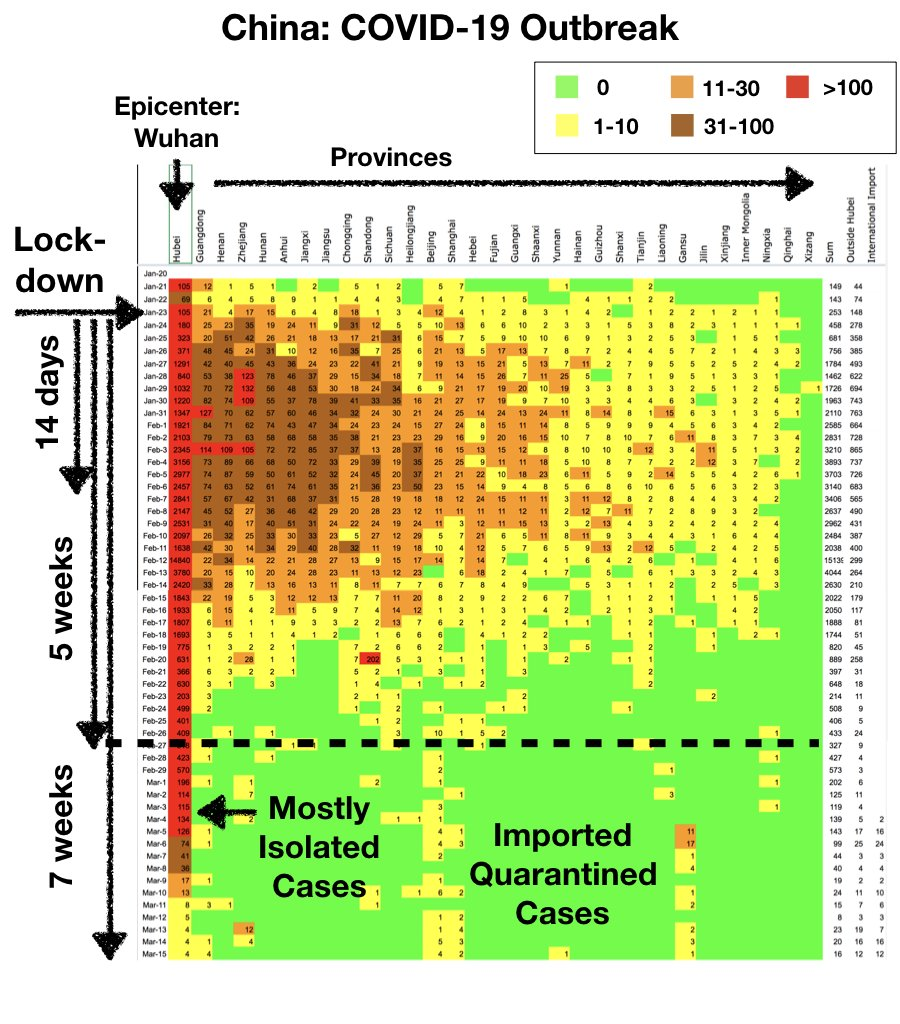
\includegraphics[scale=0.85]{ChinaDynamics.png}
\caption{Dinamica dell'epidemia in Cina che mostra il momento del contenimento e il numero di casi per ogni provincia.}
\end{centering}
\end{figure}




% \bibliography{MyCollection.bib}


\end{document}
